

\section{Weighted automata over a product of two free monoids}
\label{sec:fmp-fct}

Automata over a product of (two) free monoids are called 
\emph{transducers} in the literature and 
\index{transducer}
\code{fmp-transducers} in \vcsn,  
`\code{fmp}' stands for \emph{free monoid product}.
Their behaviours are series over~$\Ae\x\Be$, \ie weighted subsets 
of~$\Ae\x\Be$, or weighted relations from~$\Ae$ (input monoid) 
to~$\Be$ (output monoid), but looked at symmetrically. 

Transducers can also be considered as automata over the input 
alphabet with multiplicity in the semiring of (rational) series over 
the output alphabet (the equivalence between the two points of view 
is asserted by the Kleene-Sch\"utzenberger theorem).
These would be called \code{rw-transducers} in \vcsn,  
`\code{rw}' stands for \emph{rational weights}. 
They are not 
implemented in \tafkitv (\cf \sbsct{taf-ins}) but
will be in subsequent versions.

In the sequel, we denote the input monoid by~$\Ae$, the output monoid 
by~$\Be$ --- in \tafkitv, they are both alphabets of characters or 
both alphabets of integers --- 
and the weight semiring (numerical, and commutative) by~$\K$ --- in 
\tafkitv, $\B$ or~$\Z$.
We denote the transducers by \Prm{tdc} rather than by \Prm{aut}.

As automata over~$\Ae\x\Be$, \code{fmp-transducers} are 
eligible to functions listed in \secti{aut-fct} and that apply to 
all automata.
For technical reasons, functions which involve reading rational 
expressions: \FctInd{cat-E},  
\FctInd{exp-to-aut}, are not implemented in \tafkitv.
On the other hand, a number of functions are specific to transducers, 
and are described in this section.

\begin{enumerate}

\item Transformations of transducers

\begin{enumerate}
\item \Fcttra{inverse}
\item \Fcttra{transpose}
% \item \Fcttra{is-normalized}, \Fcttra{normalize}
\item \Fcttra{is-subnormalized}, \Fcttra{subnormalize}
\item \Fcttra{is-ltl}
\item \Fcttra{ltl-to-pair}
\end{enumerate}

\item Operations on transducers

\begin{enumerate}
\item \Fcttra{domain}, \Fcttra{image}, \Fcttra{w-domain}, \Fcttra{w-image}
\item \FcttraD{composition} %,\FcttraD{b-composition}
% \item \Fcttraaut{domain-restriction}, \Fcttraaut{image-restriction}
\item \Fcttraaut{evaluation}
\item \FctParD{eval}{tdc}{word}
\end{enumerate}

\item Operations on behaviours of transducers

\begin{enumerate}
    \item \FcttraD{composition-R}
%     \item \Fcttraaut{evaluation-S}
%     \item \Fcttra{inverse-R}
\end{enumerate}

% \item Transformations of transducers
% 
% \begin{enumerate}
% \item \Fcttra{realtime}
% \end{enumerate}
% 
% \item Properties and transformations of expressions
% 
% \begin{enumerate}
% \item \Fctexp{inverse-E}
% \item \Fctexp{transpose-E}
% \end{enumerate}

\end{enumerate}

\longonly{%
\begin{ComVd}{110709}
    
Fonctions pas impl�ment�es:
 \Fct{evaluation-S}.
\end{ComVd}
}%


\SetTwClPrm{\TwClOne}%
\subsection{Transformations of transducers}

\subsubsection{\Fct{inverse}}

\begin{SwClCmd}
\begin{shell}
$ \kbd{vcsn inverse t.xml > u.xml}
$
\end{shell}%
\end{SwClCmd}%
\begin{SwClTxt}
    \Prm{u.xml} realizes what is called the \emph{inverse relation} of 
    the relation realized by \Prm{t.xml}
\end{SwClTxt}%
\IndexFct{inverse}

\Prec no precondition.

\Spec
Swaps the first for the second component in the labels of the 
transitions of the transducer \Prm{t.xml} and writes the result 
in the transducer \Prm{u.xml}. 

\Comt
\Fctq{inverse}{t.xml} is kind of pivotal function and 
will have an influence on the specification of other functions.

\subsubsection{\Fct{transpose}}
\label{ssc:fmp-tra}


\begin{SwClCmd}
\begin{shell}
$ \kbd{vcsn transpose t.xml > u.xml}
$
\end{shell}%
\end{SwClCmd}%
\begin{SwClTxt}
    Computes the transposition of the transducer \Prm{t.xml}
     and writes the result 
    in the transducer \Prm{u.xml}. 
\end{SwClTxt}%

\Prec no precondition.

\Spec
\thi Builds the transposition of the underlying graph.

\thii Transposes 
the labels of the transitions thanks to the extension of the function 
\Fctp{transpose} from words to pair of words:\\
\Fctq{transpose}{(f,g)}= \code{(\Fctq{transpose}{f},\Fctq{transpose}{g})}.

% \begin{ComVd}{100607}
%     Exists probably in \vcsnv (as it is used in \code{ORR}), but not in \tafkit.
%     May be be withdrawn at the end.
% \end{ComVd}

% \subsubsection{\Fct{is-normalized}, \Fct{normalize}}
% \label{ssc:fmp-nor}%
% 
% \begin{ComVd}{100502}
%     It seems that these functions do not exist in \tafkit.
% I still mention them now in this document, for two reasons:
% 
% \thi to mark the difference with the functions with the same name 
% which are defined for automata over a free monoid (\cf 
% \sbsct{aut-nor}).
% 
% \thii it is the easiest way 
% to talk about \emph{subnormalization}.
% 
% May be withdrawn at the end.
% \end{ComVd}
% 
% 
% \begin{SwClCmd}
% \begin{shell}
% $ \kbd{vcsn is-normalized -v t.xml}
% Input is normalized
% \end{shell}%
% \end{SwClCmd}%
% \begin{SwClTxt}
%     Tells whether or not the transducer 
%        \Prm{t.xml} is normalized.
% \end{SwClTxt}%
% \IndexFctIs{normalized}
% 
% \Spec
% A transducer is normalized if it is
% % \begin{enumerate}
% %     \item  
% \thi
% \emph{proper};
% 
% %     \item  
%     \thii `letterized', \emph{in the sense} that the labels of 
% transitions are either in $(A \x \unBe)$ or in $(\unAe \x B)$;
% 
% %     \item  
%     \thiii initial and final functions take values in the weight semiring.
% % \end{enumerate}
% \clearpage 
% 
% \Comt 
% \thi   Remark the similarity with \Fctp{is-realtime} for an automaton, 
%     although a normalized transducer is not at all what is called a 
%     \emph{realtime transducer} (reserved for \code{rw-transducer}).
% 
% 
% \thii   The name is not good but classical for transducers and we do 
%     not have found a good alternative.
% 
% \medskip
% % \newpage 
% \begin{SwClCmd}
% \begin{shell}
% $ \kbd{vcsn normalize t.xml > u.xml}
% $
% \end{shell}%
% \end{SwClCmd}%
% \begin{SwClTxt}
%     Computes from \Prm{t.xml} a normalized transducer
% %     by
% %     eliminating the spontaneous transitions from a `letterized' version 
% %     of \Prm{t.xml} 
%     and writes the result in \Prm{u.xml}.
% \end{SwClTxt}%
% \IndexFct{normalize}
% 
% 
% \Prec no precondition.
% 
% \Spec 
% \begin{enumerate}
%     \item  As for \Fctp{realtime}, and for the same reason (\cf 
% \sbsct{aut-mul-rea}), one wants to `letterize' first, and then 
% eliminate the spontaneous transitions.
% 
%     \item We are to 
% `letterize' monomials such as 
% $\msp \mathtt{m = \{k\}(f,g)}\msp$
% with~$f$  in~$\Ae$ and~$g$ in~$\Be$.
% % \begin{equation}
% %     \mathtt{m = \{k\}(f,g)}\EqVrg \ee \text{with~$f$  
% % in~$\Ae$ and~$g$ in~$\Be$.}
% % \notag
% % %     \label{}
% % \end{equation}
% \begin{enumerate}
%     \item  if the monomial~$\mathtt{m}$ is of the form 
% $\mathtt{m = \{k\}(a\xmd b\xmd c,x\xmd y)}$, that is, if~$g$ is in~$\Bp$, 
% decompose it in the product of $n=\lgt{f}+\lgt{g}$  
% generators in the following way:
% \begin{equation}
%     \mathtt{(a,1)\xmd (b,1)\xmd (c,1)\xmd (\{k\}(1,x))\xmd (1,y)}
%     \notag
% %     \label{}
% \end{equation}
% 
% 
%     \item  if the monomial~$\mathtt{m}$ is of the form 
% $\mathtt{m = \{k\}(a\xmd b\xmd c,1)}$, that is,
% if~$g=\unBe$, decompose it in the product of $n=\lgt{f}$ 
% generators
% in the following way:
% \begin{equation}
%     \mathtt{(\{k\}(a,1))\xmd (b,1)\xmd (c,1)}\notag
% %     \label{}
% \end{equation}
% \end{enumerate}
% 
%     \item  create $n-1$ states between the origin and the end of the 
% transition labeled by the monomial and the~$n$ transitions such that 
% each of them is labeled by one of the generators we have computed in 
% the above decomposition, one of them being weighted.
% 
%     \item  eliminate the spontaneous transitions with a `backward' procedure.
% \end{enumerate}
% 
% \Comt
% The decomposition in~(2) may look awkward. 
% It corresponds to what we would like to get when 
% applying a function which would transform 
% \Prm{t.xml} into a \emph{realtime} \rwt .
% 

\Exam
\figur{fib} shows the left-to-right cautious Fibonacci transducer 
(\cf \cite[Example~V.1.4]{Saka03}), its inverse, and its 
transpose.\footnote{% 
   In \cite{{Saka03}}, transducers are allowed to have final 
   functions that have non-scalar values;
   thus the examples there and here have a slightly different look.}

\begin{figure}[ht]
    \centering
\PushLine
\makebox[0pt][c]{\includegraphics[scale=0.4]{figures/fib-gd.ps}}
\eee\e
\PushLine
\eee\e
\makebox[0pt][c]{\includegraphics[scale=0.4]{figures/fib-gd-inv.ps}}
\eee
\PushLine
\eee\ee
\makebox[0pt][c]{\includegraphics[scale=0.4]{figures/fib-gd-trsp.ps}}
\PushLine
\caption{The left-to-right cautious Fibonacci transducer, its 
inverse, and its transpose}
\label{fig:fib}
\end{figure}

\clearpage 
\subsubsection{\Fct{is-subnormalized}, \Fct{subnormalize}}

\begin{SwClCmd}
\begin{shell}
$ \kbd{vcsn is-subnormalized -v t.xml}
Input is not subnormalized
\end{shell}%
\end{SwClCmd}%
\begin{SwClTxt}
    Tells whether or not the transducer 
       \Prm{t.xml} is subnormalized.
\end{SwClTxt}%
\IndexFctIs{subnormalized}

\Spec
A transducer is \emph{subnormalized} if it is
\begin{enumerate}
    \item  \emph{proper};

    \item  weakly `letterized', \emph{in the sense} that the labels of 
transitions are either in $(A \x \unBe)$ or in $(\unAe \x B)$, or 
in~$(A\x B)$;

    \item  initial and final functions are \emph{scalar}, that is, take values in the weight semiring.
\end{enumerate}

\Comt 
The terminology `subnormalized' is new (introduced 
in~\cite{ClavEtAl05}) and comes from `normalized',
\index{subnormalized| see{transducer}}%
\index{transducer!subnormalized --}%
which means that the labels of 
transitions are either in $(A \x \unBe)$ or in $(\unAe \x B)$.
The terminology `normalized' is not so good, as it collides with the 
notion of normalized automata, but is widely accepted and used.
Once `normalized' is accepted, `subnormalized' is not so bad. 
Other suggestions are still welcome: no established 
terminology exists. 


\medskip
\begin{SwClCmd}
\begin{shell}
$ \kbd{vcsn subnormalize t.xml > u.xml}
$
\end{shell}%
\end{SwClCmd}%
\begin{SwClTxt}
    Computes from \Prm{t.xml} a subnormalized transducer 
%     by
%     eliminating the spontaneous transitions from a weakly 
%     `letterized' version  
%     of \Prm{t.xml} 
    and writes the result in \Prm{u.xml}.
\end{SwClTxt}%
\IndexFct{subnormalize}


\Prec no precondition.

\Spec 
\begin{enumerate}
    \item  As for \Fct{proper} above, one wants to `letterize' first, 
and then eliminate the spontaneous transitions.

    \item  
    We are to 
    `letterize' monomials such as 
    $\msp \mathtt{m = \{k\}(f,g)}\msp$
    with~$f$  in~$\Ae$ and~$g$ in~$\Be$.
%     As we have a \law automaton, we are to 
% `letterize' monomials such as
% \begin{equation}
%     \mathtt{\{k\}(f,g)}\EqVrg \ee \text{with~$f$  
% in~$\Ae$ and~$g$ in~$\Be$.}
% \notag
% %     \label{}
% \end{equation}
    
A monomial of the form 
$\mathtt{\{k\}(a\xmd b\xmd c,x\xmd y)}$ will be 
decomposed in the product of $n=\sup (\lgt{f},\lgt{g})$  
`generators' in the following way:
\begin{equation}
    \mathtt{(\{k\}(a,x))\xmd (b,y)\xmd (c,1)}
    \notag
%     \label{}
\end{equation}

    \item  create $n-1$ states between the origin and the end of the 
transition labeled by the monomial and the~$n$ transitions such that 
each of them is labeled by one of the generators we have computed in 
the above decomposition, the first one being possibly weighted.


    \item  eliminate the spontaneous transitions with a `backward' procedure.
\end{enumerate}

\Comt
The
\Fct{subnormalize} function is only a `decomposition' algorithm; it does not 
attempt to make the automaton more compact: this would be the task of 
other, and more sophisticated, algorithms.

\Exam
\figur{sbn} shows a $\Z$-transducer and its subnormalization.
Note that the transducer \code{fx1.xml} cannot be built, nor edited,
with the \FctInd{edit} function.

\begin{figure}[ht]
    \centering
\includegraphics[scale=0.5]{figures/fx1.ps}
\ee
\includegraphics[scale=0.5]{figures/fx1-sbn.ps}
\caption{A $\Z$-transducer and its subnormalization}
\label{fig:sbn}
\end{figure}

\Cave
The \Fct{subnormalize} function requires that the transducer meets 
the scalar end-function condition.
\index{condition!scalar end-function}%


% 
% \thii
% A normalized automaton \Prm{t.xml} is subnormalized and
% \Fctq{subnormalize}{t.xml} = \code{t.xml} when \Prm{t.xml} is 
% normalized. 
% 
% On the other hand, for any \Prm{t.xml}, 
% \Fctq{normalize}{\Fctq{subnormalize}{t.xml}} is likely to yield a different
% result than 
% \Fctq{normalize}{t.xml}.
% This is due to the fact that \Fctp{normalize} is
% specified in view of the function \Fctp{realtime}.


\subsubsection{\Fct{is-ltl}}


\begin{SwClCmd}
\begin{shell}
$ \kbd{vcsn is-ltl -v t.xml}
Input is letter-to-letter
\end{shell}%
\end{SwClCmd}%
\begin{SwClTxt}
    Tells whether or not the label of every transition of 
       \Prm{t.xml} is in~$A\x B$.
\end{SwClTxt}%
\IndexFctIs{ltl}%
\index{letter-to-letter| see{transducer}}%
\index{transducer!letter-to-letter --}%

% \Spec
% The description of \Fctp{is-ltl} is a specification of 
% \emph{letter-to-letter} transducers.


\subsubsection{\Fct{ltl-to-pair}}

\begin{SwClCmd}
\begin{shell}
$ \kbd{vcsn ltl-to-pair t.xml > a.xml}
$
\end{shell}%
\end{SwClCmd}%
\begin{SwClTxt}
    Transforms \Prm{t.xml} into an automaton over $(A\x B)^{*}$ with 
    weight in~$\K$ and writes the result in  
    \Prm{a.xml}. 
\end{SwClTxt}%
\IndexFct{ltl-to-pair}

\Prec \Prm{t.xml} is letter-to-letter.

\Spec
The label of every transition of \Prm{t.xml} becomes \emph{a letter} in the 
alphabet~$(A\x B)$ and the weight of the transition is kept unchanged.

\Comt
A letter-to-letter transducer and an automaton over the corresponding 
alphabet of pairs looks very much the same when they are drawn 
by the \Fct{display} function. 
But they are very different with respect to the functions which can 
be applied to them.

\begin{shell}
$ \kbd{vcsn-char-fmp-b display trx.xml}
$ \kbd{vcsn-char-fmp-b ltl-to-pair trx.xml > trx-pair.xml}
$ \kbd{vcsn-char-char-b complete trx-pair.xml \bslash| complement - > trx-pair-cmp.xml}
$ \kbd{vcsn-char-fmp-b complete trx.xml \bslash| complement - > trx-cmp.xml}
vcsn-char-fmp-b: command `complete' doesn't exist.
\end{shell}%
% $ \kbd{vcsn-char-char-b display fmp/trx-pair.xml}

\begin{figure}[ht]
    \centering
\includegraphics[scale=0.4]{figures/trx.ps}
\PushLine 
\includegraphics[scale=0.4]{figures/trx-pair.ps}
\PushLine 
\includegraphics[scale=0.4]{figures/trx-pair-cmp.ps}
\caption{A letter-to-letter transducer, its pair of characters 
version, and the complement}
\label{fig:ltl-pai}
\end{figure}

\subsection{Operations on transducers}

\subsubsection{\Fct{domain}, \Fct{image}, \Fct{w-domain}, \Fct{w-image}}
\label{ssc:fmp-dom-ima}

\begin{SwClCmd}
\begin{shell}
$ \kbd{vcsn domain t.xml > a.xml}
$
\end{shell}%
\end{SwClCmd}%
\begin{SwClTxt}
    Forgets the second component of the label \emph{and the weight} of the 
    transitions of the transducer  
    \Prm{t.xml} and writes the result in the \emph{characteristic automaton} 
    \Prm{a.xml} on~$\Ae$. 
\end{SwClTxt}%
\IndexFct{domain}

\Prec no precondition.

\medskip\medskip 
\begin{SwClCmd}
\begin{shell}
$ \kbd{vcsn image t.xml > b.xml}
$
\end{shell}%
\end{SwClCmd}%
\begin{SwClTxt}
    Forgets the first component of the label \emph{and the weight} of the 
    transitions of the transducer  
    \Prm{t.xml} and writes the result in the \emph{characteristic automaton}
    \Prm{b.xml} on~$\Be$. 
\end{SwClTxt}%
\IndexFct{image}


\Prec no precondition.

\Comt
The specification for \Fct{image} is taken so that the 
following identities hold:

\noindent 
\Fctq{image}{t.xml} = \Fctq{domain}{\Fctq{inverse}{t.xml}}
\e
and

\noindent 
\Fctq{domain}{t.xml} = \Fctq{image}{\Fctq{inverse}{t.xml}}.

\begin{figure}[ht]
    \centering
\includegraphics[scale=0.5]{figures/fx1-dom.ps}
\ee
\includegraphics[scale=0.5]{figures/fx1-im.ps}
\caption{The domain and image of \code{fx1.xml}}
\label{fig:dom-im}
\end{figure}

\Cave 
The results of \Fct{domain} and \Fct{image} could, or should, have 
been \emph{Boolean} automata.
In \tafkitv, they are automata with the same weight semiring as the 
operand.

% \thi The specification for \Fctp{domain} is taken in view of the same 
% function for the \code{rw-transducers} (\cf \sbsct{taf-ins}).

\begin{SwClCmd}
\begin{shell}
$ \kbd{vcsn w-domain t.xml > a.xml}
$
\end{shell}%
\end{SwClCmd}%
\begin{SwClTxt}
    Forgets the second component of the label and \emph{keeps the weight} of the 
    transitions of the transducer  
    \Prm{t.xml} and writes the result in the automaton
    \Prm{a.xml} on~$\Ae$. 
\end{SwClTxt}%
\index{domain@\texttt{w-domain}}%

\Prec no precondition.

\medskip\medskip 
\begin{SwClCmd}
\begin{shell}
$ \kbd{vcsn w-image t.xml > b.xml}
$
\end{shell}%
\end{SwClCmd}%
\begin{SwClTxt}
    Forgets the first component of the label and \emph{keeps the weight} of the 
    transitions of the transducer  
    \Prm{t.xml} and writes the result in the automaton
    \Prm{b.xml} on~$\Be$. 
\end{SwClTxt}%
\index{image@\texttt{w-image}}%

\Prec no precondition.

\begin{figure}[ht]
    \centering
\includegraphics[scale=0.5]{figures/fx1-wdom.ps}
\ee
\includegraphics[scale=0.5]{figures/fx1-wim.ps}
\caption{The weighted domain and image of \code{fx1.xml}}
\label{fig:dom-im}
\end{figure}


\subsubsection{\Fct{composition}, \Fct{b-composition}} %
\label{ssc:fmp-com}

As we shall see, the composition algorithms of \fmpts are defined on 
\emph{subnormalized} ones only.
\index{transducer!subnormalized --}
There are two distinct functions for the composition.
The first one, \Fct{composition}, yields a \fmpt in which the number 
of paths is preserved. 
It is the only one which makes sense for \emph{weighted} \fmpt.
The second one, \Fct{b-composition}, is reserved for \emph{Boolean} 
\fmpts, and yields a \fmpt which is simpler, but in which the number 
of paths is not preserved.


\SetTwClPrm{\TwClThree}%
\begin{SwClCmd}
\begin{shell}
$ \kbd{vcsn composition t.xml u.xml > v.xml}
$
\end{shell}%
\end{SwClCmd}%
\begin{SwClTxt}
    Realizes the composition algorithm on 
    \Prm{t.xml} and \Prm{u.xml} and writes the result in  
    \Prm{v.xml}. 
\end{SwClTxt}%
\IndexFct{composition}%


\Prec \Prm{t.xml} and \Prm{u.xml} are subnormalized, with matching 
monoids (output of \Prm{t.xml} = input of \Prm{u.xml}) and same 
weight semirings.

\Spec
The composition algorithm used in \tafkit 
is described at \sbsct{fmp-com-E}.

\Comt
When the weight semiring is not \emph{complete}, it may be the case 
that the composition is not defined, in which case the call to 
\Fct{composition} will produce an error.

% \begin{ComVd}{091222}
%     The `product' of \emph{subnormalized} transducers is a function that has to be 
%     described separatly. %(\cf \sbsct{fmp-com-E})
% 
%     
%     To tell the truth, the last time I applied this algorithm on an 
%     example (when preparing a lecture), I was not so happy with the result. I 
%     have to check it again, and I may change some details (in for out, forward 
%     closure for backward closure, such kind of things) but the general 
%     structure will remain the same.
% \end{ComVd}


\medskip\medskip 
\begin{SwClCmd}
\begin{shell}
$ \kbd{vcsn b-composition t.xml u.xml > v.xml}
$
\end{shell}%
\end{SwClCmd}%
\begin{SwClTxt}
    Realizes the Boolean composition algorithm on 
    \Prm{t.xml} and \Prm{u.xml} and writes the result in  
    \Prm{v.xml}. 
\end{SwClTxt}%
\IndexFct{b-composition}%


\Prec \Prm{t.xml} and \Prm{u.xml} are subnormalized, with matching 
monoids (output of \Prm{t.xml} = input of \Prm{u.xml}) and Boolean 
weight semiring.

\Spec
The Boolean composition algorithm is described at \sbsct{fmp-com-E} and goes 
roughly as follows: 
\begin{enumerate}
    \item  performing the `product' of \Prm{t.xml} and \Prm{u.xml}

    \item  make the result proper.
\end{enumerate}

\Exam
\figur{com-pos} shows the \Fct{b-composition} and the 
\Fct{composition} of the \fmpts \code{t1.xml} and \code{u1.xml} that 
are taken as examples at \sbsct{fmp-com-E} (\cf \figur{tra-pro} and 
\figur{com-mul}).
\begin{shell}
$ \kbd{vcsn-char-fmp-b b-composition t1.xml u1.xml \bslash| display -}
$ \kbd{vcsn-char-fmp-b composition t1.xml u1.xml \bslash| display -}
\end{shell}%
Note that the \Fct{b-composition} is not \emph{trim}.


\begin{figure}[ht]
    \centering
\includegraphics[scale=0.5]{figures/comp2.ps}
\ee
\includegraphics[scale=0.5]{figures/comp1.ps}
\caption{\Fct{b-composition} and 
\Fct{composition} of \code{t1.xml} and \code{u1.xml}}
\label{fig:com-pos}
\end{figure}


\Cave
In \tafkitv, \Fct{b-composition} and \Fct{composition} do not test 
the precondition \Fct{is-subnormalized}.
In the case where this precondition is not met, the result is not 
correct.

This error will be corrected in subsequent versions.



% \subsubsection{\Fct{domain-restriction}, \Fct{image-restriction}}
% 
% \begin{SwClCmd}
% \begin{shell}
% $ \kbd{vcsn domain-restriction t.xml a.xml > u.xml}
% $
% \end{shell}%
% \end{SwClCmd}%
% \begin{SwClTxt}
%     Computes a transducer whose domain is the intersection of the 
%     domain of \Prm{t.xml} with the language accepted by \Prm{a.xml} 
%     (and does not change the relation on this domain)
%      and writes the result in the transducer \Prm{u.xml}
% \end{SwClTxt}%
% 
% 
% \begin{ComV}
%     Reminder.
% \end{ComV}


\subsubsection{\Fct{evaluation}}
\label{ssc:fmp-eva-ltn}%

\begin{SwClCmd}
\begin{shell}
$ \kbd{vcsn evaluation t.xml a.xml > b.xml}
$
\end{shell}%
\end{SwClCmd}%
\begin{SwClTxt}
    Computes an automaton which realizes the 
    image of the series realized by \Prm{a.xml} by the relation 
    realized by \Prm{t.xml} and writes the result in  
    \Prm{b.xml}. 
\end{SwClTxt}%
\IndexFct{evaluation}


\Prec \Prm{t.xml} is subnormalized, \Prm{a.xml} is a realtime 
automaton over the input monoid of  \Prm{t.xml}, \Prm{t.xml} and 
\Prm{a.xml} have the same weight semiring.

\Spec
\Fctq{evaluation}{t.xml, a.xml} = 
\Fctq{W-image}{\Fctq{composition}{\Fctq{partial-identity}{a.xml},{t.xml}}}

\Comt
When the weight semiring is not \emph{complete}, it may be the case 
that the evaluation is not defined, in which case the call to 
\Fct{evaluation} will produce an error.

\medskip 
\subsubsection{\Fct{eval}}

\begin{SwClCmd}
\begin{shell}
$ \kbd{vcsn eval t.xml 'exp' }
fxp
\end{shell}%
\end{SwClCmd}%
\begin{SwClTxt}
    Computes an automaton which realizes the 
    image of the expression \Prm{exp} by the relation 
    realized by \Prm{t.xml} and outputs the result as the expression 
    \Prm{fxp}. 
\end{SwClTxt}%
\IndexFct{eval}


\Prec \Prm{t.xml} is subnormalized, \Prm{exp} is an expression
 over the input monoid of \Prm{t.xml}.

% \Spec
% \Fctq{eval}{t.xml, w} = 
% \Fctq{evaluation}{t.xml, \Fctq{standard}{w}}

\Comt
Just a wrapper for \Fct{evaluation}.

\Cave
In \tafkitv, the expressions \Prm{exp} and \Prm{fxp} have to be under 
the string format: the \ShortOpt{i} and \ShortOpt{o} options have no effect 
on this function.



% \begin{ComVd}{100602}
%     Reminder. 
%     It is not clear that this function should exists. 
% \end{ComVd}



\subsection{Operations on behaviours of transducers}

\subsubsection{\Fct{composition-R}}

\begin{SwClCmd}
\begin{shell}
$ \kbd{vcsn composition-R t.xml u.xml > v.xml}
$
\end{shell}%
\end{SwClCmd}%
\begin{SwClTxt}
    Computes a transducer that realizes the composition of the 
    relations realized by  
    \Prm{t.xml} and \Prm{u.xml} and writes the result in  
    \Prm{v.xml}. 
\end{SwClTxt}%
\IndexFct{composition-R}


\Prec \Prm{t.xml} and \Prm{u.xml} have matching 
monoids (output of \Prm{t.xml} = input of \Prm{u.xml}) and the same 
weight semiring.

\Spec
\Fctq{composition-R}{t.xml, u.aml} = 
\Fctq{composition}{\Fctq{subnormalize}{t.xml}, \Fctq{subnormalize}{u.xml}}

% \begin{ComV}
%     Problems with the definition (on non-complete weight semiring). 
% \end{ComV}
% 



% \subsubsection{\Fct{evaluation-S}}
% 
% \begin{SwClCmd}
% \begin{shell}
% $ \kbd{vcsn evaluation-S t.xml a.xml > b.xml}
% $
% \end{shell}%
% \end{SwClCmd}%
% \begin{SwClTxt}
%     Computes an automaton which realises the series which is the 
%     image of the series realized by \Prm{a.xml} by the relation 
%     realized by \Prm{t.xml} and writes the result in  
%     \Prm{b.xml}. 
% \end{SwClTxt}%
% \IndexFct{evaluation-S}
% 
% 
% \Prec \Prm{t.xml} is any transducer, \Prm{a.xml} is any 
% automaton over the input monoid of \Prm{t.xml}, \Prm{t.xml} and 
% \Prm{a.xml} have the same weight semiring.
% 
% \Spec
% \Fctq{evaluation-S}{t.xml, a.xml} = 
% \Fctq{evaluation}{\Fctq{subnormalize}{t.xml},\Fctq{realtime}{a.xml}}

\longonly{%
\medskip\medskip
\begin{ComVd}{110710}
    \Fct{evaluation-S} pas impl�ment�e.
\end{ComVd}
}%


% \begin{ComV}
%     Problems with the definition (on non-complete weight semiring). 
% \end{ComV}


% \subsection{Transformations of transducers}
% 
% \subsubsection{\Fct{realtime}}
% 
% \begin{SwClCmd}
% \begin{shell}
% $ \kbd{vcsn realtime t.xml > a.xml}
% $
% \end{shell}%
% \end{SwClCmd}%
% \begin{SwClTxt}
%     Implements the Kleene--Sch\"utzenberger Theorem, that is,
%     transforms \Prm{t.xml} into an equivalent automaton over $\Ae$ with 
%     weight in~$\KRat\Be$ and writes the result in  
%     \Prm{a.xml}. 
% \end{SwClTxt}%
% 
% 
% \Prec \Prm{t.xml} is normalized.
% 
% \Spec
% To be described.
% 
% \begin{ComV}
%     \tha 
%     Problem with the name: we have a kind of overloading of the 
%     meaning of `realtime' in case of transducers. Could be \Fctp{fmp-to-rw} as 
%     well. 
%     
%     \thb
%     The result may be not defined (on non-complete weight semiring). 
% \end{ComV}


% \subsection{Properties and transformations of expressions}
% 
% \subsubsection{\Fct{inverse-E}}
% \subsubsection{\Fct{transpose-E}}
% 
% 






\SetTwClPrm{\TwClOne}%
%%%%%%%%%%%%%%%%%%%%%%
\endinput
